\documentclass[11pt,letterpaper]{article}
\usepackage[utf8]{inputenc}
\usepackage[spanish, es-tabla]{babel}
\usepackage[version=3]{mhchem}
\usepackage[journal=jacs]{chemstyle}
\usepackage{amsmath}
\usepackage{amsfonts}
\usepackage{amssymb}
\usepackage{makeidx}
\usepackage{xcolor}
\usepackage[stable]{footmisc}
\usepackage[section]{placeins}
\usepackage{longtable}
\usepackage{array}
\usepackage{xtab}
\usepackage{multirow}
\usepackage{colortab}
\usepackage{siunitx}
\sisetup{mode=text, output-decimal-marker = {,}, per-mode = symbol, qualifier-mode = phrase, qualifier-phrase = { de }, list-units = brackets, range-units = brackets, range-phrase = --}
\DeclareSIUnit[number-unit-product = \;] \atmosphere{atm}
\DeclareSIUnit[number-unit-product = \;] \pound{lb}
\DeclareSIUnit[number-unit-product = \;] \inch{"}
\DeclareSIUnit[number-unit-product = \;] \foot{ft}
\DeclareSIUnit[number-unit-product = \;] \yard{yd}
\DeclareSIUnit[number-unit-product = \;] \mile{mi}
\DeclareSIUnit[number-unit-product = \;] \pint{pt}
\DeclareSIUnit[number-unit-product = \;] \quart{qt}
\DeclareSIUnit[number-unit-product = \;] \flounce{fl-oz}
\DeclareSIUnit[number-unit-product = \;] \ounce{oz}
\DeclareSIUnit[number-unit-product = \;] \degreeFahrenheit{\SIUnitSymbolDegree F}
\DeclareSIUnit[number-unit-product = \;] \degreeRankine{\SIUnitSymbolDegree R}
\DeclareSIUnit[number-unit-product = \;] \usgallon{galón}
\DeclareSIUnit[number-unit-product = \;] \uma{uma}
\DeclareSIUnit[number-unit-product = \;] \ppm{ppm}
\DeclareSIUnit[number-unit-product = \;] \eqg{eq-g}
\DeclareSIUnit[number-unit-product = \;] \normal{\eqg\per\liter\of{solución}}
\DeclareSIUnit[number-unit-product = \;] \molal{\mole\per\kilo\gram\of{solvente}}
\usepackage{cancel}
\usepackage{graphicx}
\usepackage{lmodern}
\usepackage{fancyhdr}
\usepackage[left=3.17cm,right=3.17cm,top=2.54cm,bottom=2.54cm]{geometry}
\usepackage{listings}
\usepackage{textcomp}
\usepackage{graphicx}

\setlength\parindent{0pt}
\usepackage[backend=bibtex,style=chem-acs,biblabel=dot]{biblatex}
\addbibresource{Mendeley.bib}

\renewcommand{\rmdefault}{phv}
\renewcommand{\sfdefault}{phv}

\usepackage{titlesec}
\usepackage{enumitem}
\titleformat*{\section}{\bfseries\large}
\titleformat*{\subsection}{\bfseries\normalsize}

\usepackage{float}
\floatstyle{plaintop}
\newfloat{anexo}{thp}{anx}
\floatname{anexo}{Anexo}
\restylefloat{anexo}
\restylefloat{figure}

\usepackage[margin=10pt,labelfont=bf]{caption}
\usepackage{todonotes}
\usepackage[colorlinks=true, 
            linkcolor = black,
            urlcolor  = black,
            citecolor = black,
            anchorcolor = blue]{hyperref}

%%%%%%%%%%%%%%%%%%%%%%%%%%%%%%%%%%%%%%%%%%%%%%%%%%%%%%%%%%%%%%%%%%%%%%%%%%%%%%%%%%%%%%%%%

\begin{document}
\pagestyle{plain}

\begin{center}
\textbf{\LARGE{Simulation of Smoke}}\\
	\textbf{\large{By Aman Sachan}}\\
	\textbf{\large{University of Pennsylvania}}\\
\end{center}

%%%%%%%%%%%%%%%%%%%%%%%%%%%%%%%%%%%%%%%%%%%%%%%%%%%%%%%%%%%%%%%%%%%%%%%%%%%%%%%%%%%%%%%%%

\section{Overview} 

This is an implementation of a smoke simulator based on the paper titled \href{http://physbam.stanford.edu/~fedkiw/papers/stanford2001-01.pdf}{"Visual Simulation of Smoke"}.
\newline
\textbf{ \href{https://vimeo.com/268137702}{Main Demo} }

%%%%%%%%%%%%%%%%%%%%%%%%%%%%%%%%%%%%%%%%%%%%%%%%%%%%%%%%%%%%%%%%%%%%%%%%%%%%%%%%%%%%%%%%%

\section{Demos}
\textbf{grid Resolution} = 64*64*64; \newline
\textbf{fluidDensity} = 1.0; \newline
\textbf{Ambient Temperature} = 0.0; \newline
\textbf{buoyancyAlpha} is a measure of Gravity's effect on the smoke particles. \newline
\textbf{buoyancyBeta} is a measure of the Buoyancy effect due to temperature difference.

\subsection{Smoke Sim, 3 Sources, Vorticity 0.1}

\href{https://vimeo.com/268137848}{Demo Video}

\subsection{Smoke Sim, 1 Source, Vorticity 0.1}

\href{https://vimeo.com/268137975}{Demo Video}

\subsection{Smoke Sim, 1 Source, Vorticity 0.5}

\href{https://vimeo.com/268137940}{Demo Video}

%%%%%%%%%%%%%%%%%%%%%%%%%%%%%%%%%%%%%%%%%%%%%%%%%%%%%%%%%%%%%%%%%%%%%%%%%%%%%%%%%%%%%%%%%

\section{Features}

\section{Implementation Details}

\subsection{Advection}

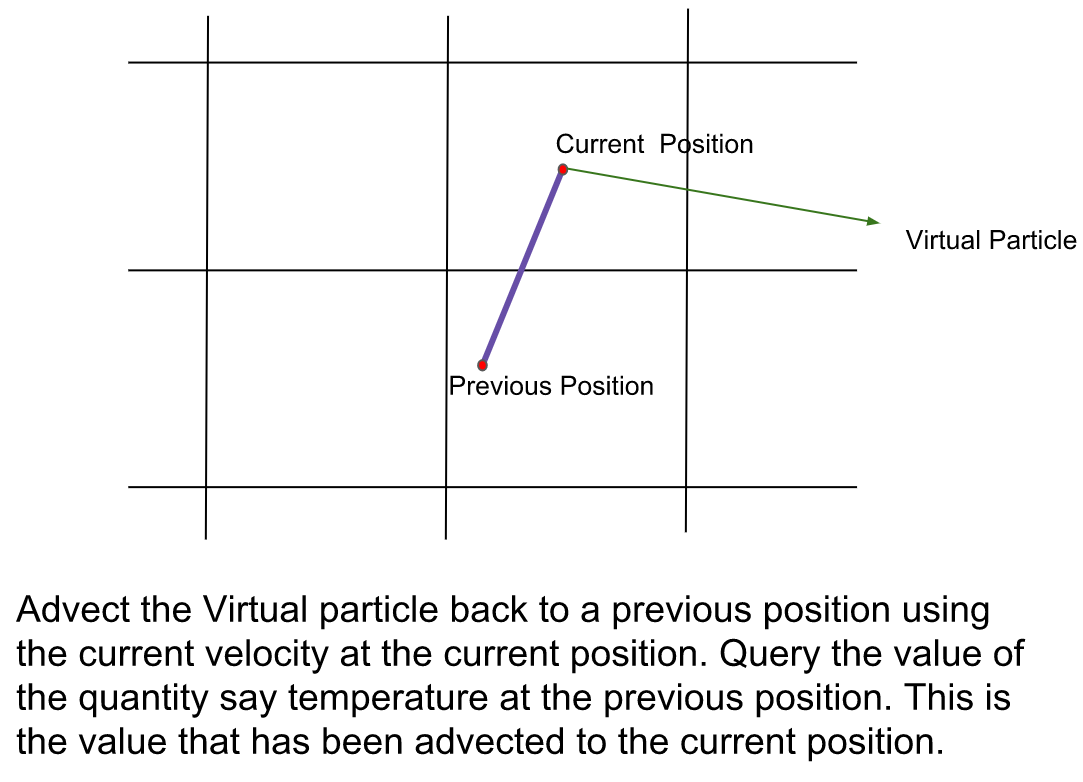
\includegraphics[width=\textwidth]{Advection.png}

Advection is being calculated in a semi-lagrangian fashion: \newline
	We are trying to calculate the value of some quantity 'q' at some position 'currentPosition' \newline
	\hspace{10mm} $\rightarrow$ Determine the currentPosition
	\newline \newline         
	
    Treat the quantity q as being stored in some imaginary particle (particles are a Lagrangian concept). Advection just says we are going to move the quantity q using some imaginary particle from its previous position to its new position (think diffusion). \newline
	\hspace{10mm} $\rightarrow$ "currState = prevState"
	\newline \newline
    
Because Advection deals with imaginary particles and not actual particles, when we retrieve the 'prevState' we get an averaged out value because every timestep we average quantities during the projection face when we calculate the velocity at the center of the cell
	\newline \newline
    For example advecting Temperature is done like so:
    
    \begin{lstlisting}
    vec3 currentPosition = getCenter(i,j,k); // Get closest grid cell center
    
    // Extrapolate the rewoundPosition by moving the current position along 
    // the current velocity by deltaT
    vec3 rewoundPosition = getRewoundPosition(currentPosition);
    
    //Get interpolated Temperature at point rewoundPosition
    double newTemperature = getTemperature(rewoundPosition); 
    
    target.mT(i,j,k) = newTemperature;
    \end{lstlisting}
    
\subsection{Projection}

	The projection step is used to calculate the new velocity at every grid cell $(u^(n+1))$ and 
	store an interpolated value at every face of the grid cell.
	\newline \newline
	This velocity that we compute for every grid cell is supposed to be divergence free to maintain
	the incompressibility of the fluid (which is an assumption we use to heavily simply the navier 
	stokes equations).
	\newline \newline
    The new velocity $u^{(n+1)}$ is calculated using 'pressure projection' which we solve using the 
	Conjugate Gradient Algorithm: \newline
	\hspace{10mm} $\rightarrow$ Solve Ap = d for pressure, where p is pressure, A is the matrix of the divergence of the gradient, and d is the divergence. \newline
	\hspace{10mm} $\rightarrow$ MAp = Md, where M is very close to the inverse of A and so MA is basically an identity matrix. \newline
	\hspace{10mm} $\rightarrow$ Therefore, p = Md; (This is the PCG (preconditionedConjugateGradient) method) \newline
	\hspace{10mm} $\rightarrow$ Construct d \newline
	\hspace{10mm} $\rightarrow$ Solve for p \newline
    \newline
	This pressure is used to get the gradient of p which is used to calculate the new velocity $u^{(n+1)}$
	\newline
    Subtract pressure from our velocity and save in target

\subsection{Bouyancy}

Buoyancy is based on this formula: \newline
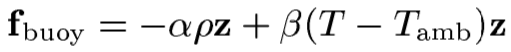
\includegraphics[width=13cm]{Buoyancy.png} \newline
where 
\textbf{Alpha} which is a measure of Gravity's effect on the smoke particles, \newline
\textbf{Beta} is a measure of the Buoyancy effect due to temperature difference, \newline
\textbf{z} is a vector that points in the upwards direction, \newline
\textbf{rho} is the density of the fluid at that point in space, \newline
\textbf{T} is the temperature of the fluid at that point in space, \newline
\textbf{$T_exp{amb}$} is the ambient room temperature.

\subsection{Vorticity Confinement}

The Vorticity confinement force is defined as: \newline
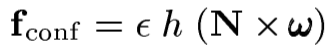
\includegraphics[width=10cm]{vorticityConfinementForce.png} \newline

where \textbf{epsilon} $>0$ is used to control the amount of small scale detail added back into the flow field, \newline
\textbf{h} is the spatial discretization to guarantee an appropriate level of accuracy, \newline

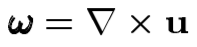
\includegraphics[width=8cm]{vorticity.png} \newline
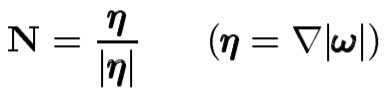
\includegraphics[width=8cm]{gradient.png} \newline
	
\end{document}
